\documentclass[11pt]{article}
\usepackage[utf8]{inputenc}
\usepackage[brazilian]{babel}
\usepackage{graphicx}
\usepackage[a4paper, top={.4in}, bottom={.65in}]{geometry}
\usepackage{subfig}
\usepackage{makecell}
\usepackage{textcomp}
\usepackage{gensymb}
\usepackage{tikz}

\begin{document}
\begin{center}
  \textbf{Experimento 05 -- PSI-3212} \\
  Natanael Magalhães Cardoso, nUSP: 8914122
\end{center}

\vspace{5mm}

\subsection*{Item 1.a}

\begin{figure}[h!]
  \centering
  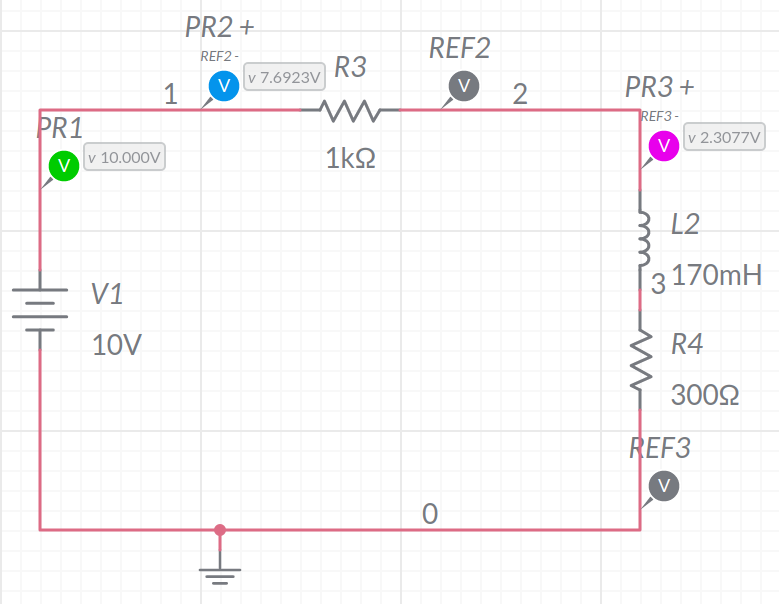
\includegraphics[width=.62\textwidth]{fig/1a}
  \caption{Diagrama do circuito}
\end{figure}

\begin{table}[h!]
  \centering
  \begin{tabular}{|c|c|c|}
    \hline
    \multicolumn{3}{|c|}{Circuito DC}                            \\
    \hline
    V\textsubscript{E} & V\textsubscript{R} & V\textsubscript{B} \\
    \hline
    10V                & 7.6923V            & 2.3077V            \\
    \hline
  \end{tabular}
  \caption{Valores simulados de tensão}
\end{table}

\subsection*{Item 1.b}

Os valores obtidos satisfazem a segunda lei de Kirchhoff, pois
$ V_{E} = V_{R} + V_{B} $

\subsection*{Item 1.c}

% \begin{figure}[h!]
%   \centering
%   \subfloat{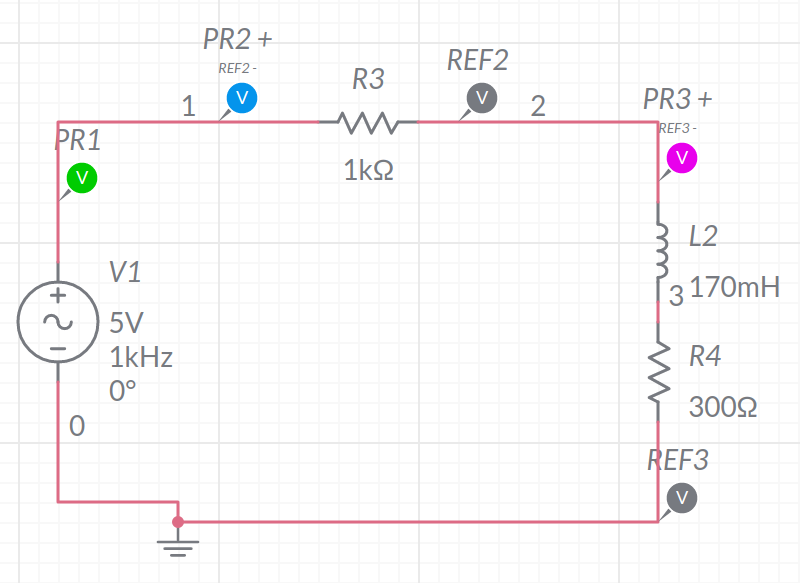
\includegraphics[width=.46\textwidth]{fig/1c.png}}
%   \qquad
%   \subfloat{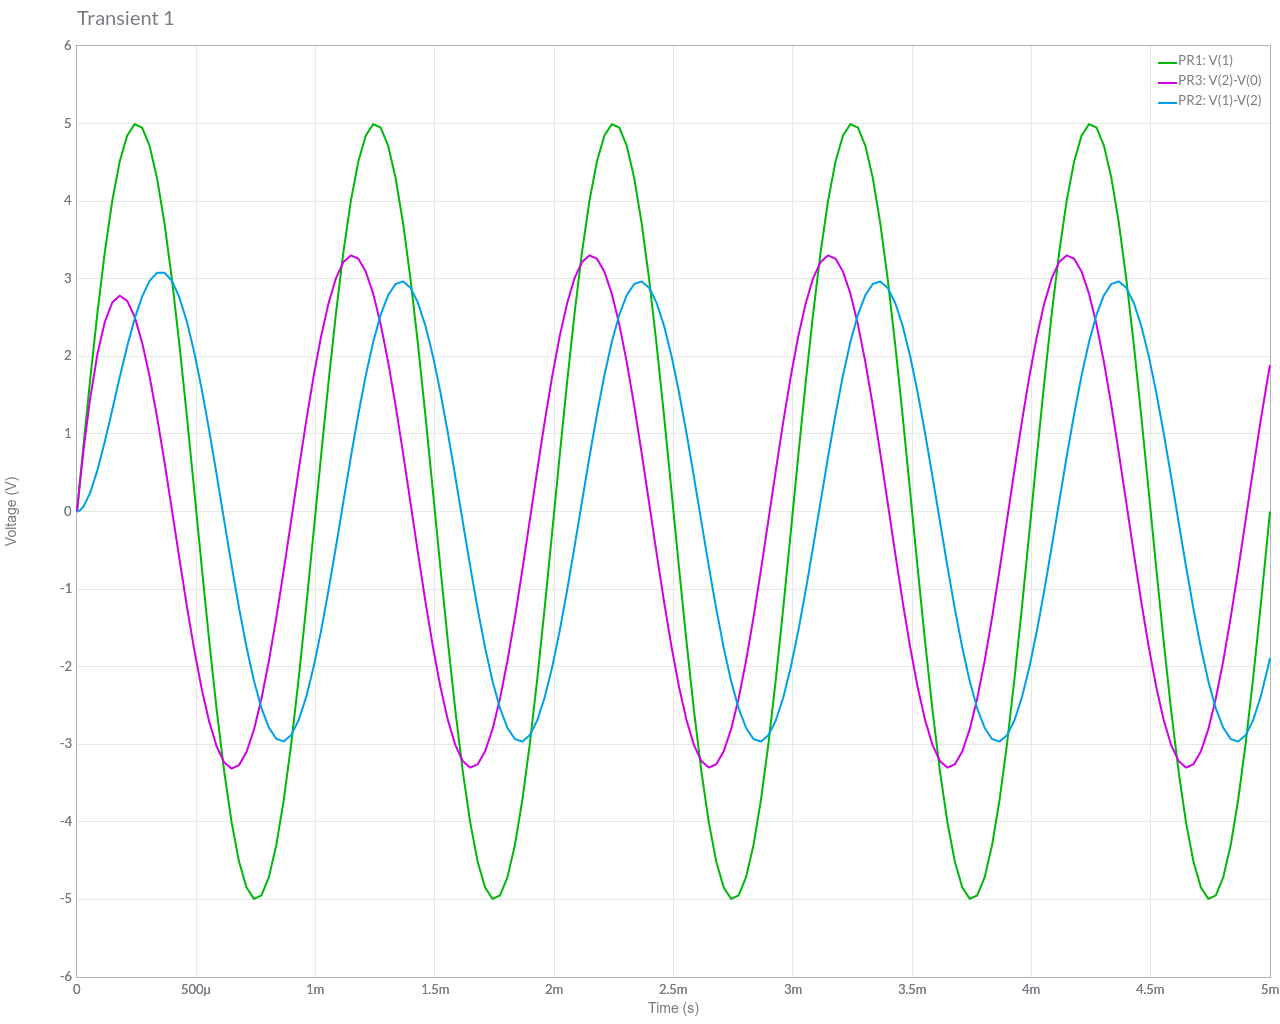
\includegraphics[width=.46\textwidth]{fig/1c_graph.png}}
% \end{figure}

\begin{figure}[h!]
  \centering
  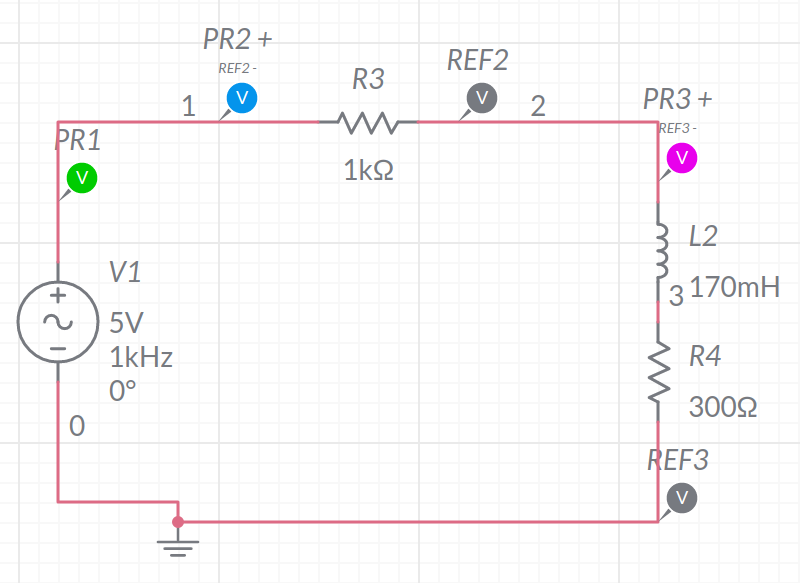
\includegraphics[width=.62\textwidth]{fig/1c}
  \caption{Diagrama do circuito}
  \label{fig:circ-1c}
\end{figure}

\pagebreak

\begin{figure}[h!]
  \centering
  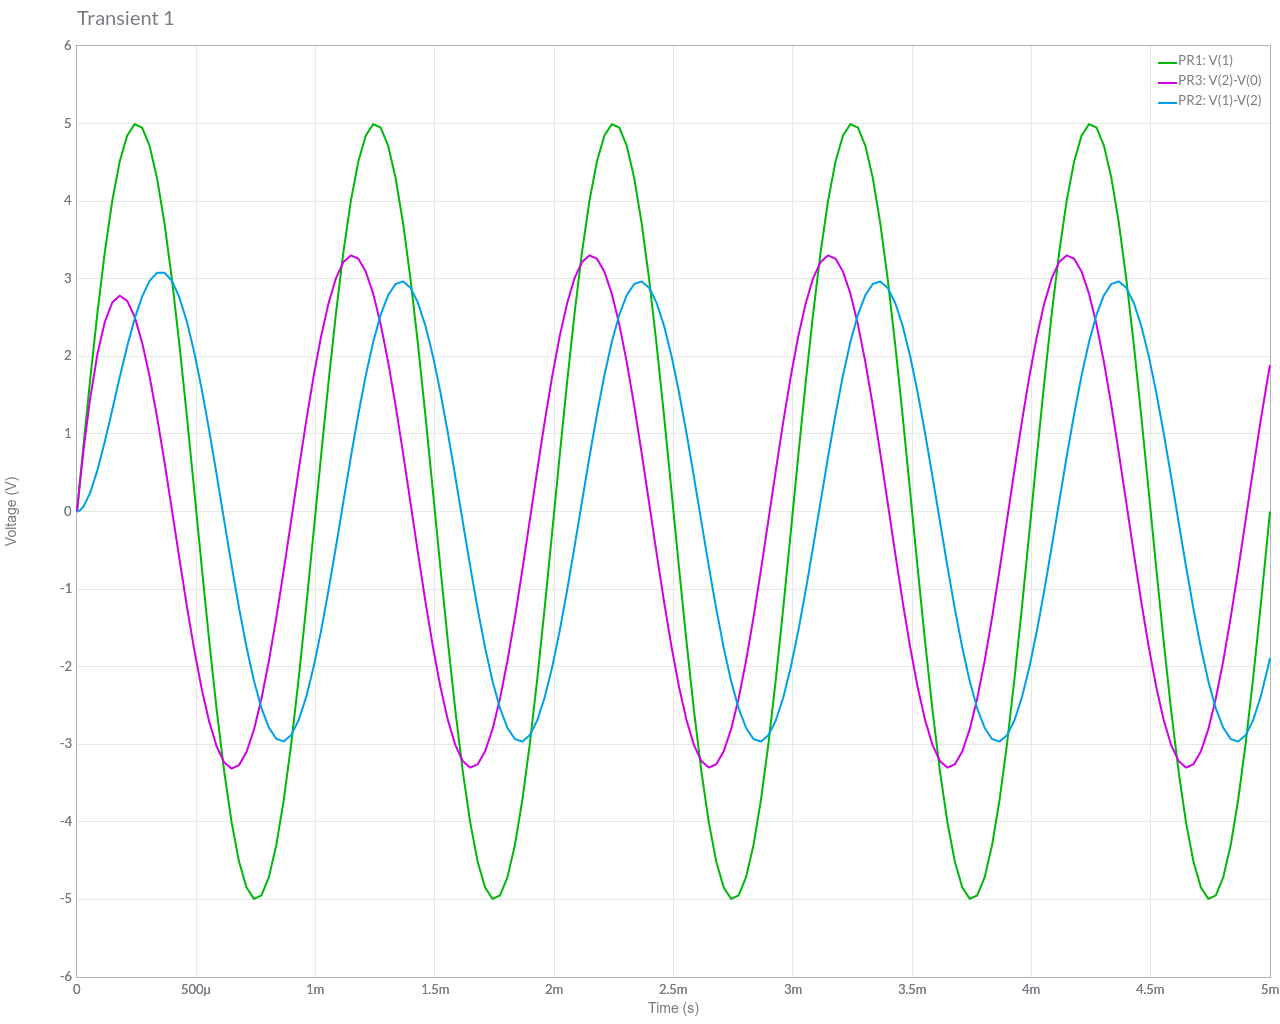
\includegraphics[width=.8\textwidth]{fig/1c_graph}
  \caption{Simulação do circuito da figura \ref{fig:circ-1c}.}
\end{figure}

\begin{table}[h!]
  \centering
  \begin{tabular}{|c|c|c|}
    \hline
    \multicolumn{3}{|c|}{Circuito AC ($V_{p}$)}                  \\
    \hline
    V\textsubscript{E} & V\textsubscript{R} & V\textsubscript{B} \\
    \hline
    4.9852V            & 2.9593V            & 3.2979V            \\
    \hline
  \end{tabular}
  \caption{Tensão de pico em E, R e B.}
\end{table}

\subsection*{Item 1.d}

Pelo gráfico abaixo, percebe-se que a curva $V_{R} + V_{B}$ é coincidente com a curva $V_{E}$. Isso significa que a soma das tensões instantâneas de $V_{R}$ e $V_{B}$ do circuiuto são sempre iguais a $V_{E}$. Portanto, para este circuito, a Segunda Lei de Kirchhoff é válida. Mas isso não se aplica quando se analisa apenas a tesão de pico.

\begin{figure}[h!]
  \centering
  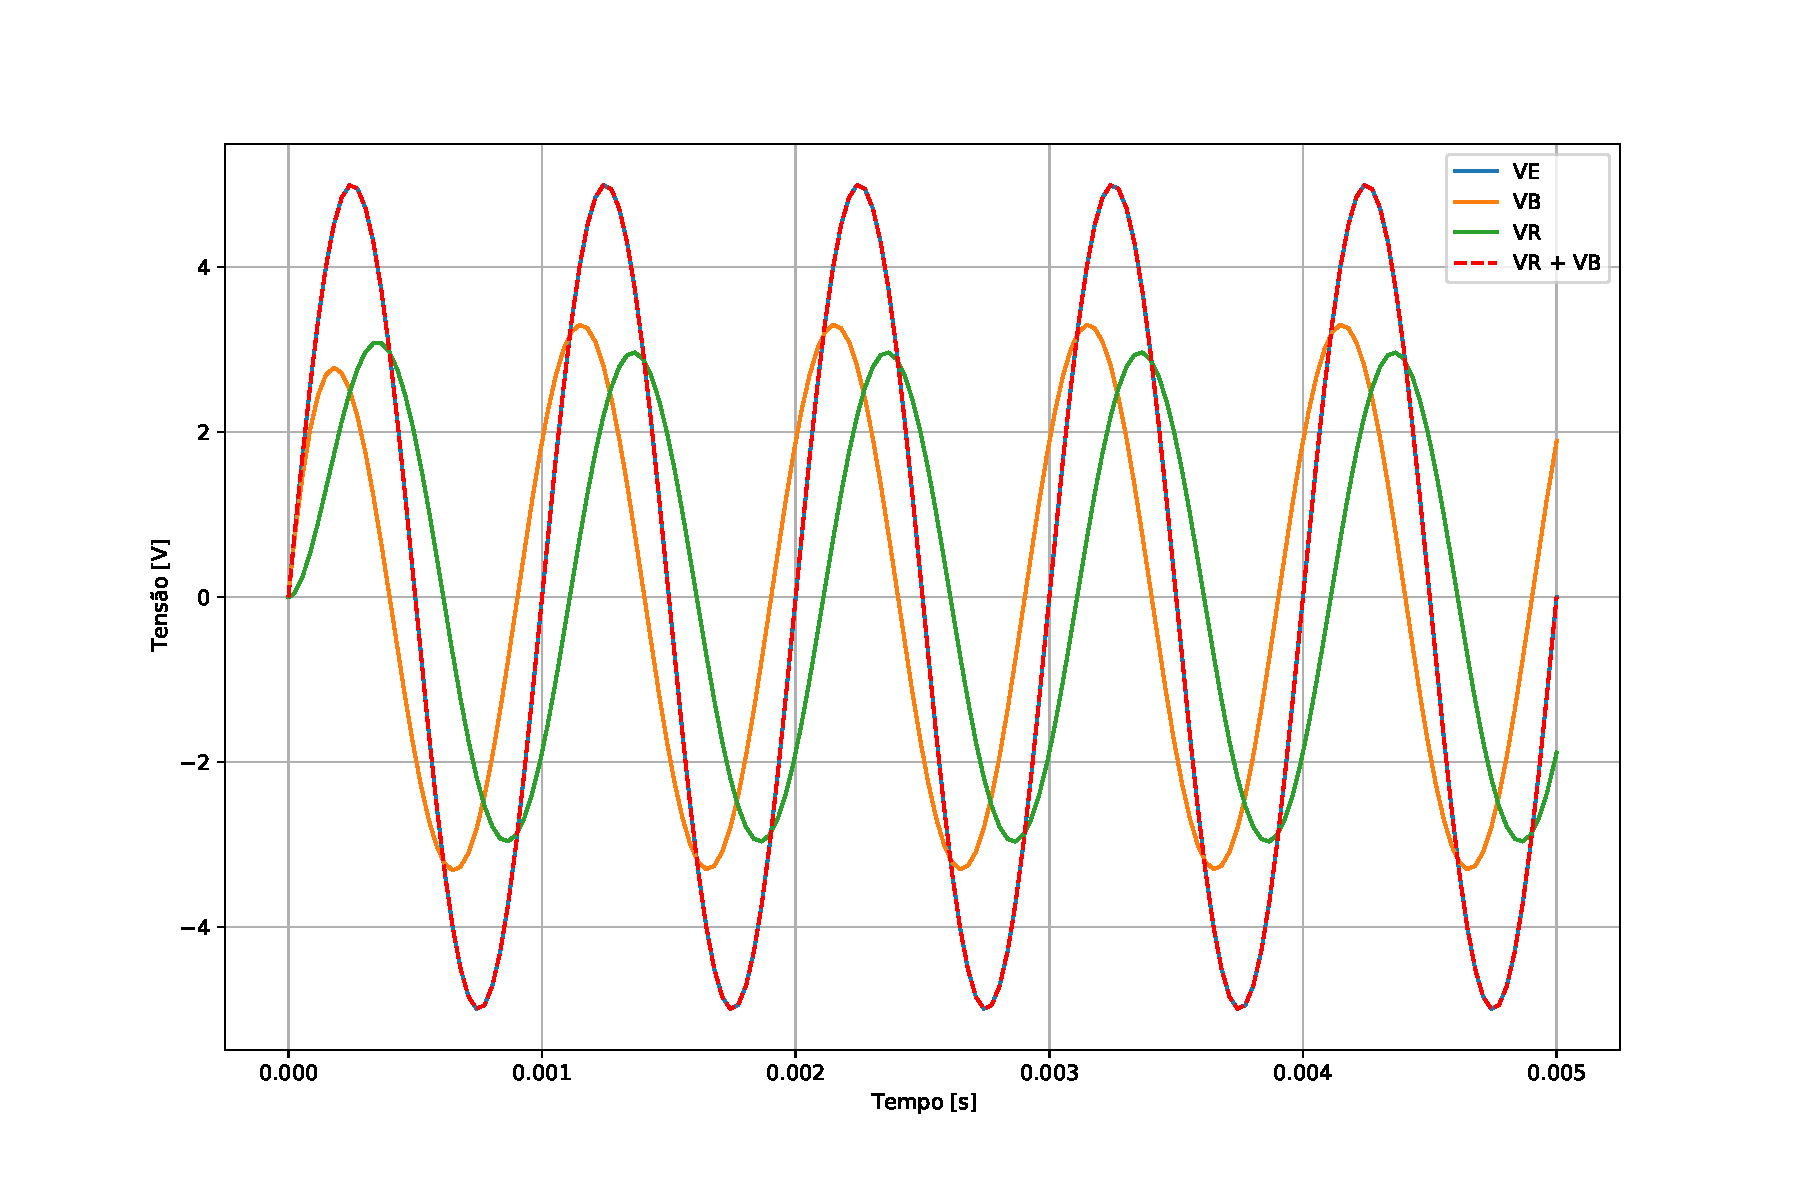
\includegraphics[width=.88\textwidth]{fig/1d.pdf}
  \caption{Simulação incluindo $V_{R} + V_{B}$.}
\end{figure}

\pagebreak

\subsection*{Item 2}

\begin{figure}[h!]
  \centering
  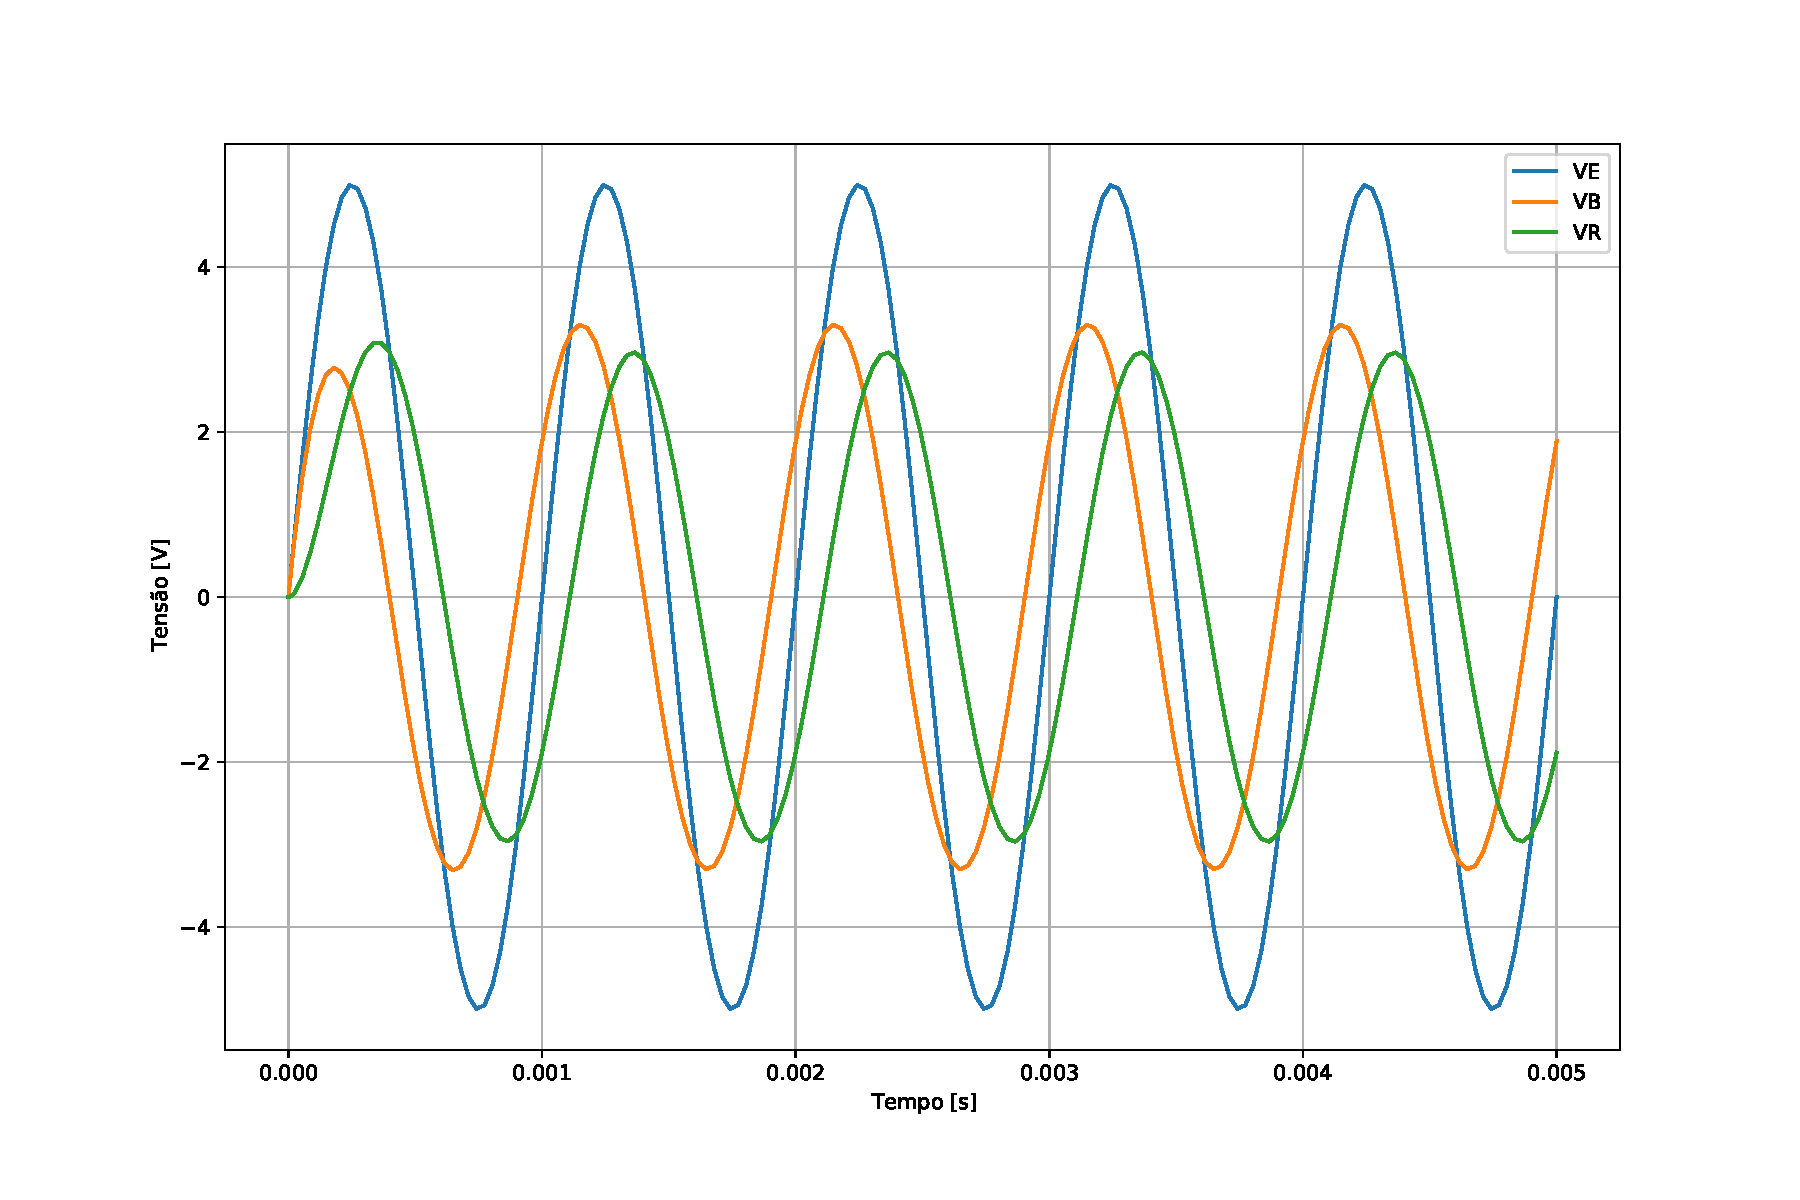
\includegraphics[width=.88\textwidth]{fig/2.pdf}
  \caption{Simuação das tensões $V_{E}$, $V_{B}$ e $V_{R}$.}
  \label{fig:2}
\end{figure}

\subsection*{Item 2.a}

\begin{table}[h!]
  \centering
  \begin{tabular}{|c|c|c|c|c|}
    \hline
    t [s]                  & $V_{E}$ [V] & $V_{B}$ [V] & $V_{R}$ [V] & $V_{B} + V_{R}$ [V] \\
    \hline
    $1.9689 \cdot 10^{-6}$ & 0.0619      & 0.0615      & 0.0004      & 0.0619              \\
    $8.5382 \cdot 10^{-5}$ & 2.5555      & 2.0259      & 0.5296      & 2.5555              \\
    $2.1038 \cdot 10^{-4}$ & 4.8459      & 2.7158      & 2.1301      & 4.8459              \\
    $5.2288 \cdot 10^{-4}$ & -0.7163     & -2.2905     & 1.5741      & -0.7163             \\
    $8.0413 \cdot 10^{-4}$ & -4.7135     & -1.9288     & -2.7847     & -4.7135             \\
    \hline
  \end{tabular}
  \caption{Pontos escolhidos}
\end{table}

\begin{figure}[h!]
  \centering
  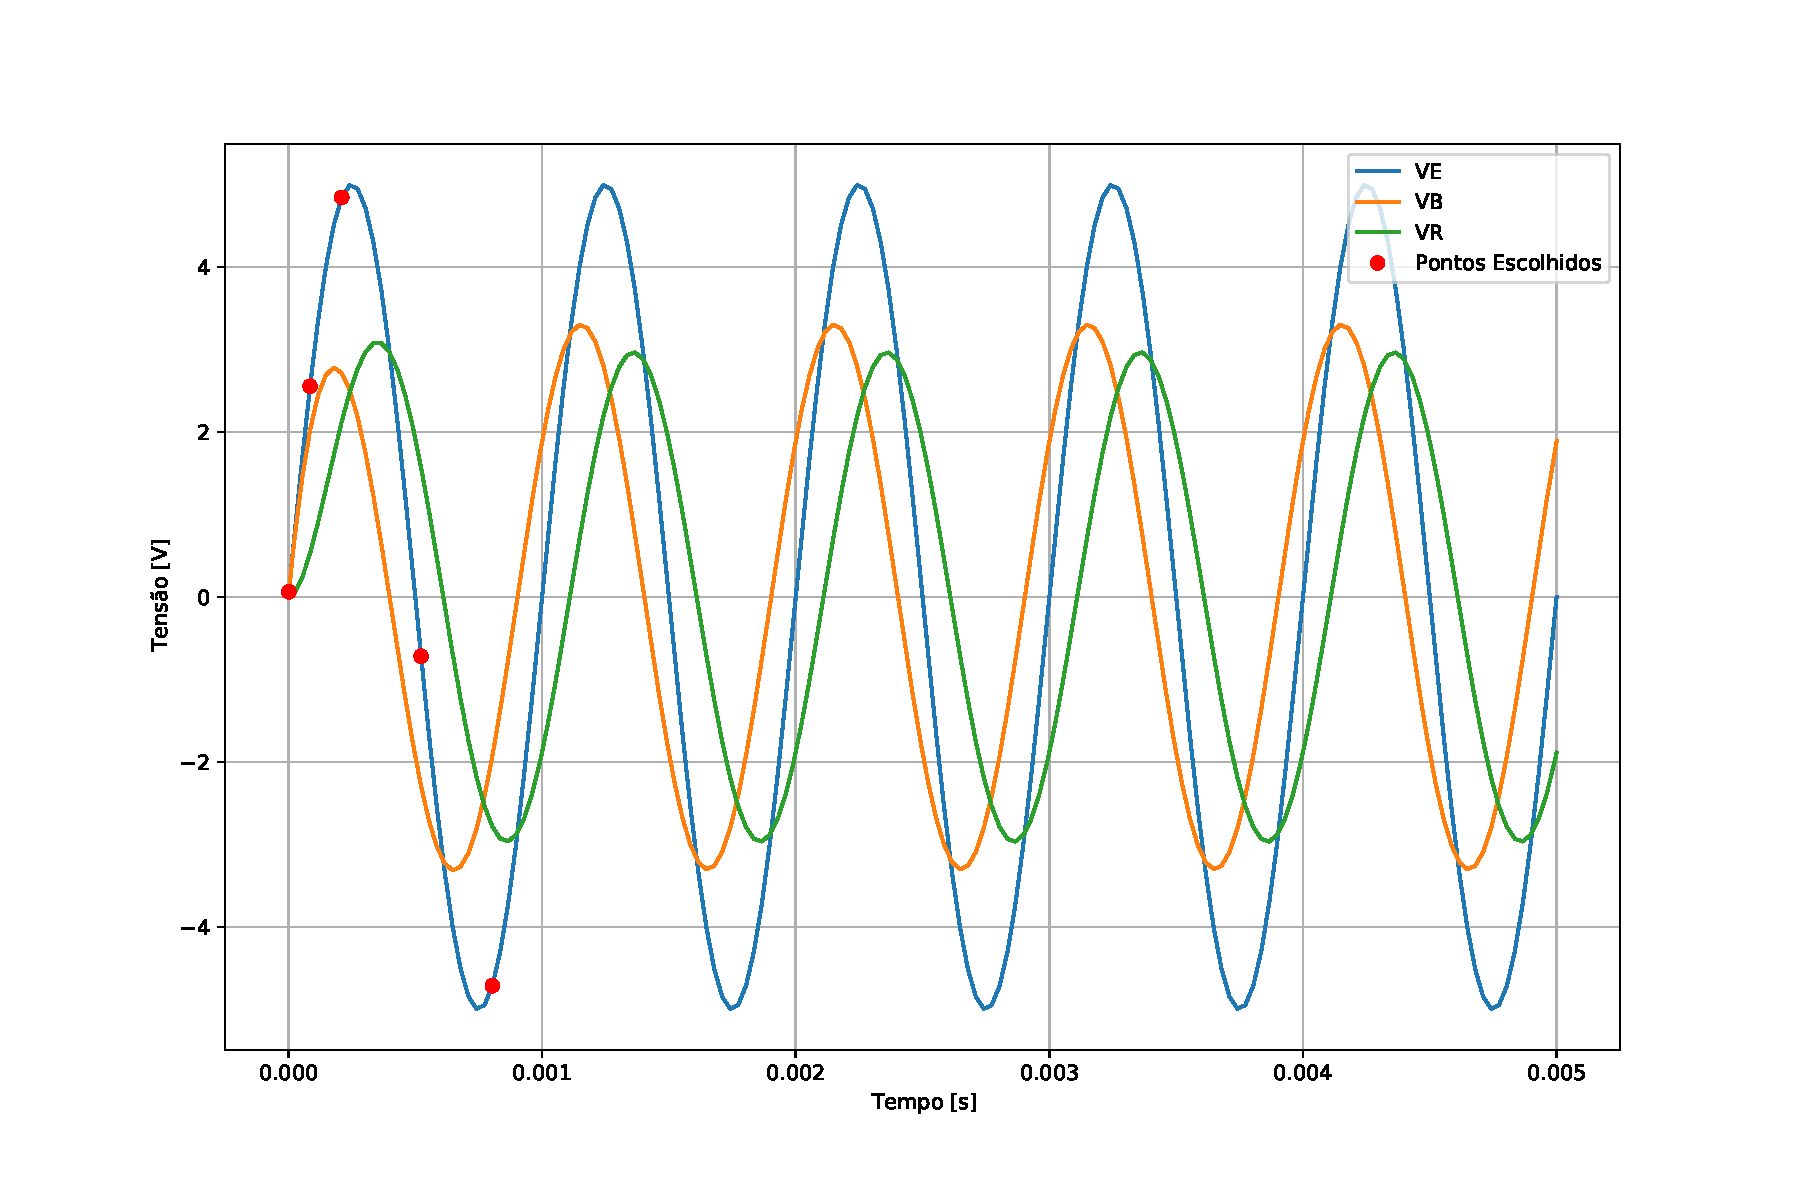
\includegraphics[width=.9\textwidth]{fig/2a}
  \caption{Visualização dos pontos escolhidos no gráfico da figura \ref{fig:2}.}
\end{figure}

\subsection*{Item 2.b}

\begin{figure}[h!]
  \centering
  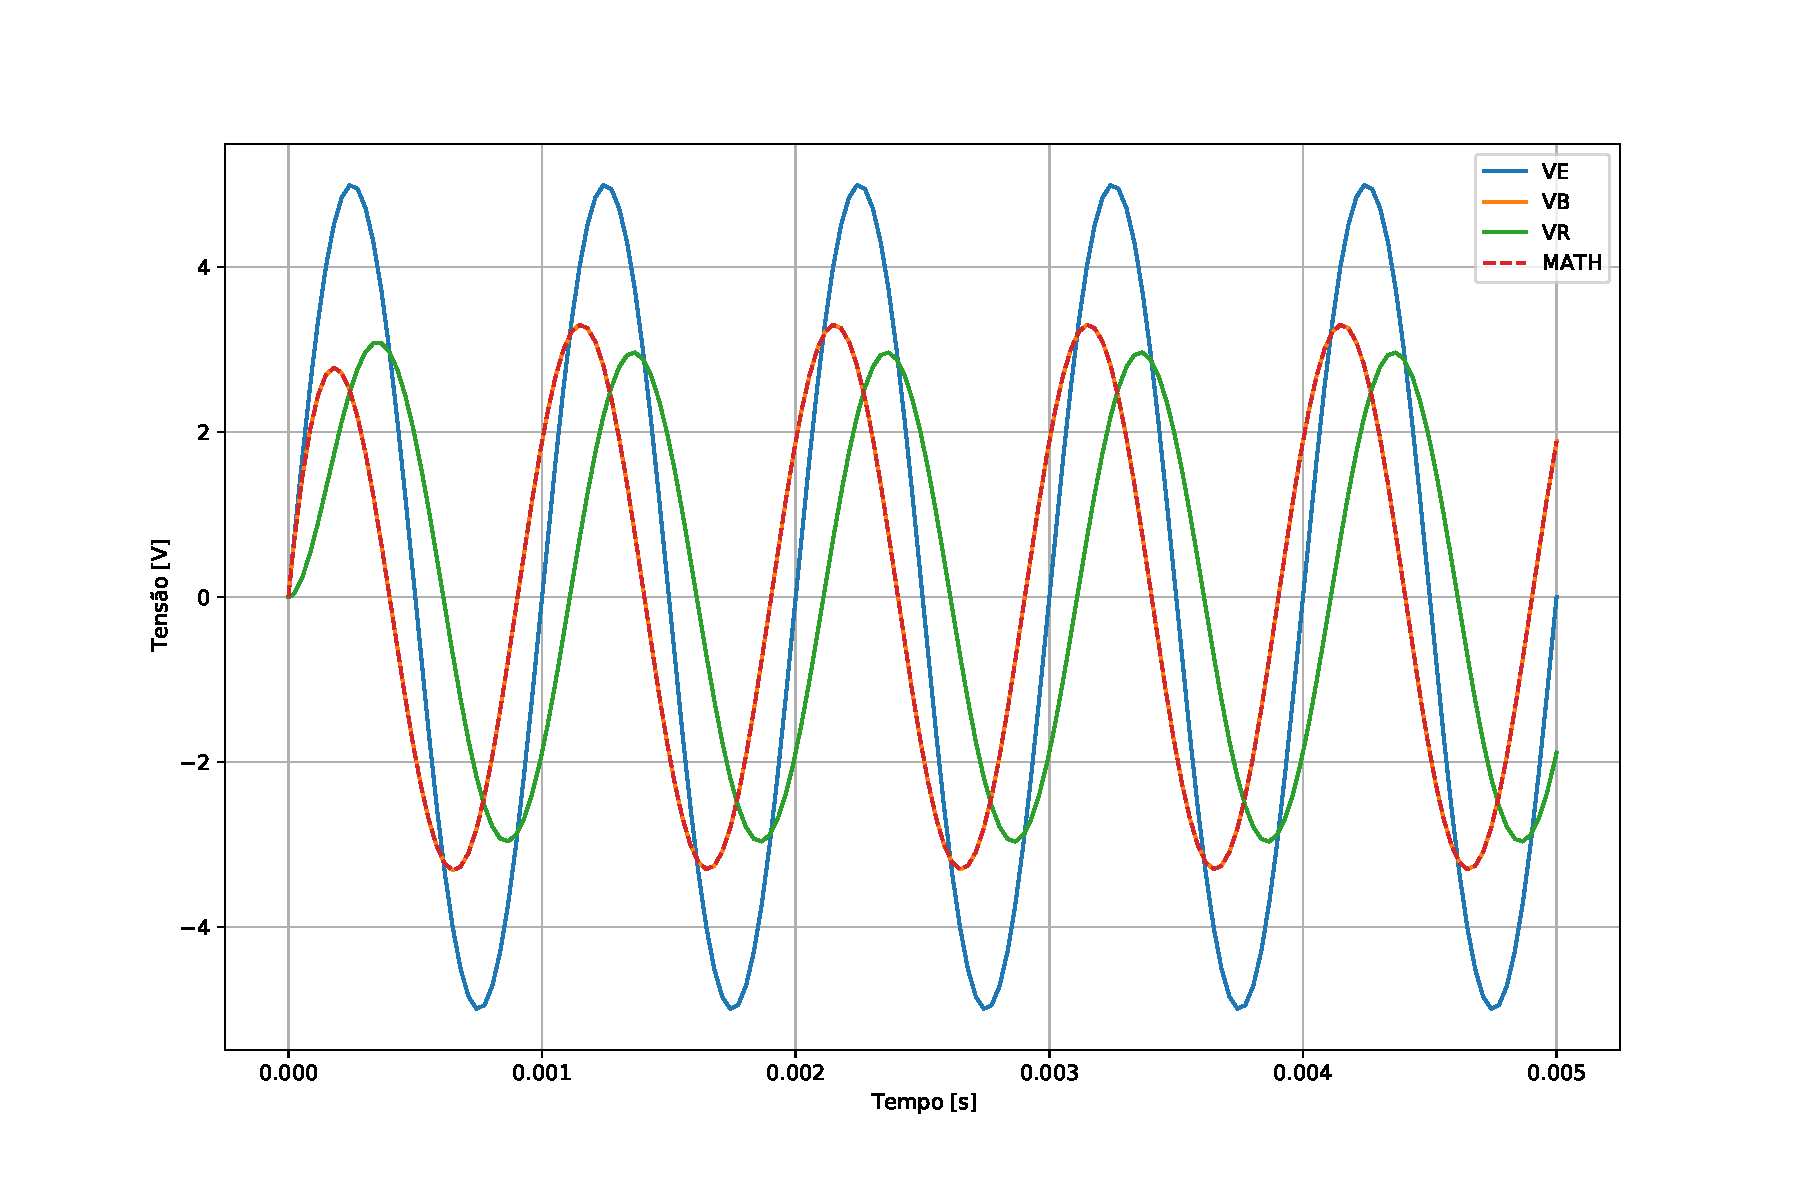
\includegraphics[width=.88\textwidth]{fig/2b.pdf}
  \caption{Simulação com a curva $MATH$.}
\end{figure}

\subsection*{Item 2.c}

A curva $MATH = V_{E} - V_{R}$ é coincidente com a curva $V_{B}$.

\subsection*{Item 2.d}

É possível concluir que a Segunda Lei de Kirchhoff não se aplica às tensões de pico, mas sim às tensões instantâneas nos circuitos com fase.

\pagebreak

\subsection*{Item 3.a}

\begin{table}[h!]
  \centering
  \begin{tabular}{|c|c|c|c|c|c|}
    \hline
    Frequência [Hz] & $V_{E}$ [V] & $V_{R}$ [V] & $V_{B}$ [V] & \makecell{Fase [\textdegree]          \\ $(V_{R} \rightarrow V_{E})$} & \makecell{Fase [\textdegree] \\ $(V_{B} \rightarrow V_{E})$} \\
    \hline
    100             & 4.9970      & 3.8208      & 2.2154      & -4.6971                      & 14.901 \\
    500             & 4.9952      & 3.5459      & 2.1815      & -22.376                      & 38.350 \\
    1k              & 4.9900      & 2.9627      & 3.2979      & -39.408                      & 34.904 \\
    \hline
  \end{tabular}
  \caption{Parâmetros para determinação dos fasores.}
\end{table}

\subsection*{Item 3.b}

\begin{table}[h!]
  \centering
  \begin{tabular}{|c|c|c|c|}
    \hline
    Fasor             & $f$ [Hz]      & Forma Polar & Forma Cartesiana \\
    \hline
    $\widehat{V}_{E}$ & \makecell{100                                  \\500\\1 k} &\makecell{4.9970                                        \\ 4.9952 \\ 4.9900}                                      & \makecell{4.9970                                        \\ 4.9952 \\ 4.9900}           \\
    \hline
    $\widehat{V}_{R}$ & \makecell{100                                  \\500 \\1 k} &\makecell{$3.8208e^{-4.6971\degree}$                    \\ $3.5459e^{-22.376\degree}$ \\ $2.9627e^{-39.408\degree}$} & \makecell{$3.8208\cos(-4.6971\degree) + j3.8208\sin(-4.6971\degree)$                    \\ $3.5459\cos(-22.376\degree) + j3.5459\sin(-22.376\degree)$ \\  $2.9627\cos(-39.408\degree) + j2.9627\sin(-39.408\degree)$}           \\
    \hline
    $\widehat{V}_{B}$ & \makecell{100                                  \\500 \\1 k} & \makecell{ $2.2154e^{14.901\degree}$                     \\$2.1815e^{38.350\degree}$ \\$3.2979e^{34.904\degree}$}   & \makecell{$2.2154\cos(14.901\degree) + j2.2154\sin(14.901\degree)$                    \\  $2.1815\cos(38.350\degree) + j2.1815\sin(38.350\degree)$ \\ $3.2979\cos(34.904\degree) + j3.2979\sin(34.904\degree)$}           \\
    \hline
  \end{tabular}
  \caption{Representação fasorial.}
\end{table}

\subsection*{Item 4.a e 4.c}

\begin{table}[h!]
  \centering
  \begin{tabular}{|c|c|c|c|}
    \hline
    Frequência & $V_{E}$ [V] & $V_{R}$ [V] & $V_{B}$ [V] \\
    \hline
    100 Hz     & 4.9970      & 3.8204      & 1.2151      \\
    500 Hz     & 4.9902      & 3.5495      & 2.1783      \\
    1 kHz      & 4.9881      & 3.2979      & 2.9622      \\
    \hline
  \end{tabular}
  \caption{Tensão de Pico.}
\end{table}

\begin{table}[h!]
  \centering
  \begin{tabular}{|c|c|c|c|c|c|}
    \hline
    Frequência & $V_{E}$ [V] & $V_{R}$ [V] & $V_{B}$  [V] & $\theta_{E}$     & $\theta_{B}$     \\
    \hline
    100 Hz     & 3.5334      & 2.7014      & 0.8592       & $3.9800\degree$  & $16.5850\degree$ \\
    500 Hz     & 3.5286      & 2.5099      & 1.5403       & $22.3847\degree$ & $60.7405\degree$ \\
    1 kHz      & 3.5271      & 2.3320      & 2.0950       & $34.9023\degree$ & $74.4725\degree$ \\
    \hline
  \end{tabular}
  \caption{Tensão RMS.}
\end{table}

\subsection*{Item 4.b}

\begin{center}
  \begin{tikzpicture}[>=stealth,x=35pt,y=35pt]
    \draw[->,thick] (0,0) -> (4.5,0);
    \draw[->,thick] (0,0) -> (0,3.5);
    \draw[->,rotate=34.9023,green!60!black,thick] (0,0) -- (4.9881,0) node [above] {\tiny $V_{E} = 4.9881$ V};
    \draw[->,rotate=74.4725,blue,thick] (0,0) -- (2.9622,0) node [above,xshift=3] {\tiny $V_{B} = 2.9622$ V};
    \draw[->,red,thick] (0,0) -- (3.2979,0) node [above] {\tiny $V_{R} = 3.2979$ V};

    \draw[->,blue] (.5,0) arc(0:74.4725:.5) node [xshift=15,yshift=12,rotate=55] {\color{blue} \tiny $74.4725\degree$};
    \draw[->,green!60!black] (.9,0) arc(0:34.9023:.9) node [xshift=21,yshift=-7] {\color{green!60!black} \tiny $34.9023\degree$};
  \end{tikzpicture}
\end{center}

\subsection*{Item 5}

\begin{table}[h!]
  \centering
  \begin{tabular}{|c|c|c|c|c|c|}
    \hline
    $f$ [Hz] & $V_{B}$ [V] & $V_{R}$ [V] & \makecell{Fase [\textdegree]                                                 \\ ($V_{B} \rightarrow V_{R}$)} & $I_{B}$ [mA] \textsuperscript{$\dagger$} & $Z_{B}$ [$\Omega$] \textsuperscript{$\ddagger$} \\
    \hline
    100      & 1.1252      & 3.8226      & 160.399                      & 3.8226 & $294.3546 e^{\pm j160.399\degree}$   \\
    200      & 1.3984      & 3.8658      & 144.429                      & 3.8658 & $361.7362 e^{\pm j144.429\degree}$   \\
    500      & 2.1818      & 3.5448      & 119.269                      & 3.5448 & $615.4931 e^{\pm j119.269\degree}$   \\
    1 k      & 3.2975      & 2.9638      & 105.689                      & 2.9638 & $1112.5919 e^{\pm j105.689\degree}$  \\
    2 k      & 4.2869      & 1.9344      & 97.982                       & 1.9344 & $2216.1394 e^{\pm j97.982\degree}$   \\
    5 k      & 4.8479      & 0.8620      & 93.222                       & 0.8620 & $5624.0139 e^{\pm j93.222\degree}$   \\
    10 k     & 4.9472      & 0.4371      & 91.6143                      & 0.4371 & $11318.2338 e^{\pm j91.6143\degree}$ \\
    \hline
  \end{tabular}
  \caption{Resultados das simulações e cálculo de $I_{B}$ e $Z_{B}$.}
  \label{tab:5a}
\end{table}

$\dagger$ \, Calculado usando $I_{B} = \frac{V_{B}}{Z_{B}}$.

$\ddagger$ \, Calculado usando $Z_{B} = |Z_{B}|e^{j\theta_{B}}$, com os valores de $|Z_{B}|$ na tabela \ref{tab:5b}.

\vspace{2mm}

\begin{table}[h!]
  \centering
  \begin{tabular}{|c|c|c|c|c|c|}
    \hline
    $f$ [Hz] & $|Z_{B}| = R\frac{V_{B}}{V_{R}}$ \\
    \hline
    100      & 294.3546                         \\
    200      & 361.7362                         \\
    500      & 615.4931                         \\
    1 k      & 1112.5919                        \\
    2 k      & 2216.1394                        \\
    5 k      & 5624.0139                        \\
    10 k     & 11318.2338                       \\
    \hline
  \end{tabular}
  \caption{Cálculos intermediários para a tabela \ref{tab:5a}.}
  \label{tab:5b}
\end{table}

\begin{figure}[h!]
  \centering
  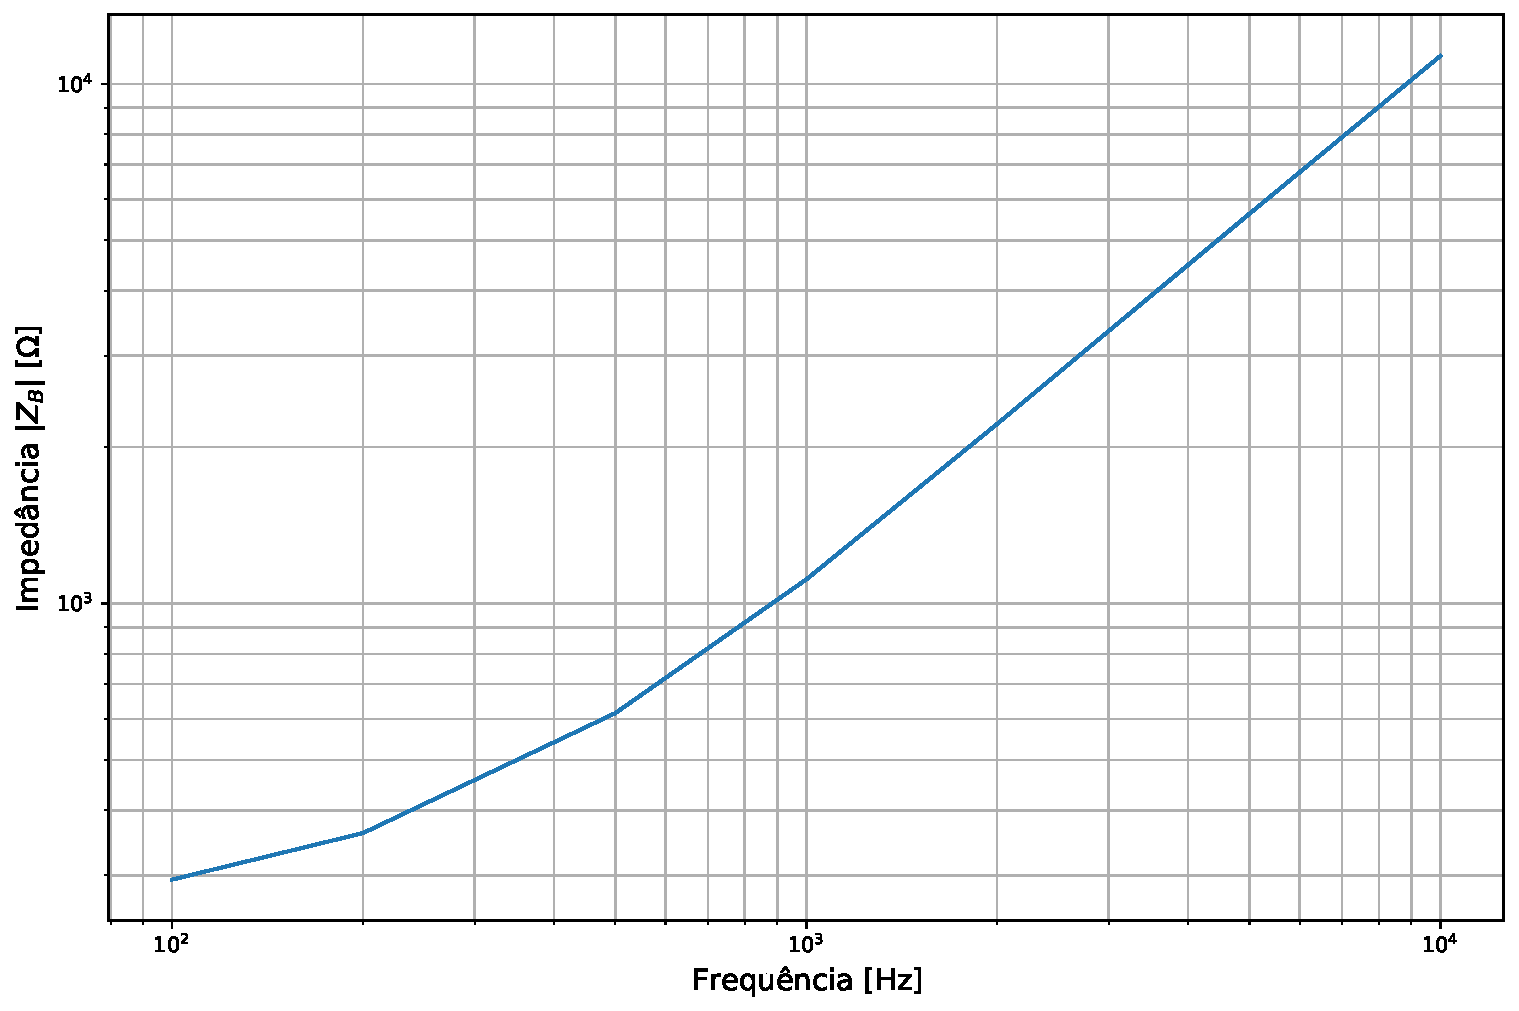
\includegraphics[width=.9\textwidth]{fig/5a}
  \caption{Gráfico Módulo da Impedância x Frequência usando a tebela \ref{tab:5b}.}
  \label{fig:5a}
\end{figure}

\pagebreak

\begin{figure}[h!]
  \centering
  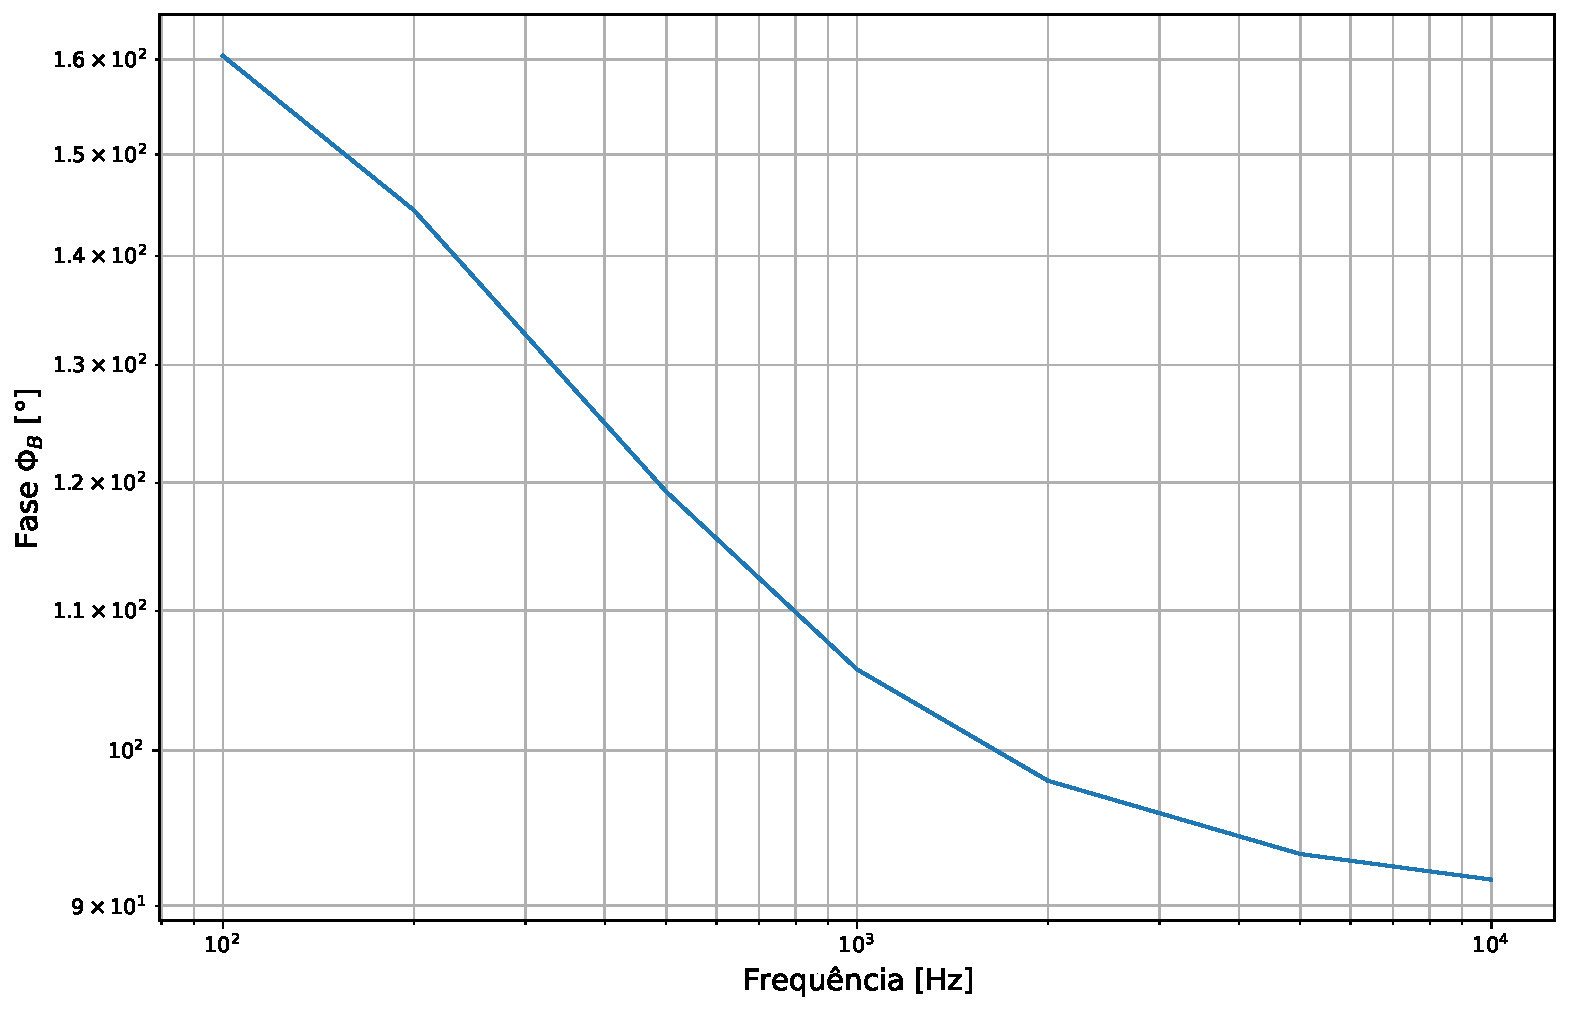
\includegraphics[width=.9\textwidth]{fig/5b}
  \caption{Gráfico Fase x Frequência usando a tebela \ref{tab:5a}.}
  \label{fig:5a}
\end{figure}

\end{document}
